\documentclass[a4paper, fontsize=14pt]{article}
\usepackage{scrextend}
\usepackage{indentfirst, fancyhdr, amsfonts, mathtools, amssymb}
\usepackage{titlesec} %работа с рубрикацией
\usepackage{tocloft} %настройки оглавления
\usepackage[T2A]{fontenc}
\usepackage[utf8x]{inputenc}
\usepackage[russian]{babel}
\usepackage{hyperref} %кликабельное оглавление
\usepackage[left=3.7cm,right=2cm,top=2cm,bottom=2cm]{geometry}
\usepackage{tempora} %настраиваем шрифт типа TNR                                   
\usepackage{newtxmath} %делаем шрифт формул похожим на TNR
\usepackage{caption}
\usepackage{listings}
\usepackage{ucs}
\lstset{
  columns=fullflexible,
  breaklines=true,
}
\linespread{1}
\setcounter{page}{4} %в зависимости от того, какой по счёту страницей должно быть оглавление!

%НАСТРОЙКИ ОГЛАВЛЕНИЯ
\renewcommand{\cftsecaftersnum}{.} %точки после номеров разделов и подразделов в оглавлении
\renewcommand{\cftsubsecaftersnum}{.}
\renewcommand{\cftsecfont}{\normalfont} %разделы в оглавлении пишутся обычным (не жирным) шрифтом
\renewcommand{\cftsecpagefont}{\normalfont} %соответствующие им страницы тоже
\renewcommand{\cftsecleader}{\cftdotfill{\cftdotsep}} %расставляем точки между названиями разделов и их страницами
\addto\captionsrussian{\renewcommand\contentsname{СОДЕРЖАНИЕ}} %хотим, чтобы слово "Содержание" писалось капсом
\renewcommand{\cfttoctitlefont}{\hfil\bfseries} %слово СОДЕРЖАНИЕ по центру жирным
\renewcommand{\cftaftertoctitle}{\hfill}

%НАСТРОЙКИ РУБРИКАЦИИ
\titleformat*{\section}{\center\bf} %названия разделов и подразделов по середине жирным шрифтом
\titleformat*{\subsection}{\center\bf}
\titlelabel{\thetitle.\quad} %название раздела и его номер отделены точкой

%НАСТРОЙКИ БИБЛИОГРАФИИ
\addto\captionsrussian{\renewcommand\refname{СПИСОК ЛИТЕРАТУРЫ}} %хотим, чтобы слова "Список литературы" писались капсом
\makeatletter
\renewcommand{\@biblabel}[1]{#1.} %хотим, чтобы в списке литературы номера источников писались в формате "No. <...>", а не "[No] <...>"
\makeatother

\begin{document}

Типы граничных условий для волнового уравнения.

Первого рода:
\begin{equation}
  \begin{cases}
    \frac{\partial^2 u}{\partial t^2} = a^2 \frac{\partial^2 u}{\partial x^2} + f(x, t) \quad &0 < x < l, \quad t > 0 \\
    u(0, t) = \phi_0(t), & x = 0, \quad t > 0 \\
    u(l, t) = \phi_1(t), & x = l, \quad  t > 0 \\
    u(x, 0) = \psi_1(x), & 0 \leq x \leq l, \quad t = 0 \\
    \frac{\partial u(x, 0)}{\partial t} = \psi_2(x), & 0 \leq x \leq l, \quad  t = 0
  \end{cases}
\end{equation}

Конечно-разностная схема для волнового уравнения (шаблон изображен на рисунке \ref{fig:yavnaya_template}):
\begin{equation}
  \frac{u_j^{k+1} - 2 u_j^k + u_j^{k-1}}{\tau^2} = a^2 \frac{u_{j+1}^k - 2 u_j^k + u_{j-1}^k}{h^2} + f_j^k
\end{equation}
\begin{equation}
  u_j^{k+1} = 2 u_j^k - u_j^{k-1} + C ( u_{j+1}^k - 2 u_j^k + u_{j-1}^k )+ \tau^2 f_j^k, \quad C = a^2 \frac{\tau^2}{h^2}
\end{equation}
\begin{figure}[h!]
  \begin{center}
    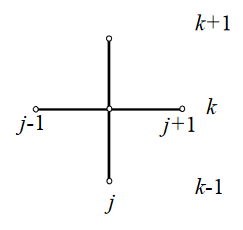
\includegraphics{src/явная схема.png}
  \end{center}
  \caption[]{шаблон явной схемы}
  \label{fig:yavnaya_template}
\end{figure}

В схеме необходимо знать $u_j^{k-1}$ и $u_j^k$ при $j = 1, \dots, N-1$ и $k = 1, 2, \dots$ на нижних временных слоях.
Для $k=1$ получаем:
\begin{equation}
  u_j^0 = \psi_1(x_j), \quad j = 0, \dots, N
\end{equation}

Для определения $u_j^1$ можно воспользоваться аппроксимацией второго начального условия.
\begin{equation}
  \frac{u_j^1 - u_j^0}{\tau} = \psi_2(x_j)
\end{equation}
\begin{equation}
  u_j^1 = \psi_1(x_j) + \tau \cdot \psi_2(x_j)
\end{equation}

Но точность можно увеличить, выбрав больше членов разложения ряда Тейлора:
  \begin{equation*}
    u_j^1 = \psi_1(x_j) + \tau \cdot \psi_2(x_j) + \frac{a^2 \tau^2}{2} \cdot \psi_1'' (x_j) 
  \end{equation*}

% \subsection*{Вывод}
% В результате проделанной лабораторной работы был изучен теоретический материал необходимый для решения поставленных задач по численному решению систем линейных алгебраических уравнений с использованием различных прямых методов и для каждой поставленной задачи написана вычислительная программа на языке программирования С++.
% \newpage
% \subsection*{Список литературы}
% \begin{enumerate}
%     \item Бахвалов Н.С., Жидков Н.П., Кобельков Г.М. Численные методы: Бином, 2018. – 636 с. 
%     \item Калиткин Н.Н. Численные методы, 2-е издание: БХВ-Петербург, 2014. – 592 с.
%     \item Самарский А.А., Гулин А. В. Численные методы: Учеб, пособие для вузов, — М.: Наука. Гл. ред. физ-мат. лит., 1989.— 432 с.
% \end{enumerate}
% \newpage
% \subsection*{Приложение}
% Весь код выложен в github-репозитории по ссылке: 

% \url{https://github.com/sultanovMF/Numerical-Methods-Lab}

\end{document}


